% Author: PokMan Ho pok.ho19@imperial.ac.uk
% Script: method.tex
% Desc: MRes thesis methods section
% Input: none
% Output: none
% Arguments: 0
% Date: Apr 2020

\documentclass[../thesis.tex]{subfiles} %% use packages & commands as this main file

\begin{document}
\section{Methodology}

The minimalist model used was composed by two players/ecological engines and three finite carbon pools (Fig.\ref{modelInWord}).  Photocells and bacterial decomposers were the two engines powering the interactions.  Both engines were sharing all but one different type of interaction, which is the carbon source.  Photocell gained carbon from the external unlimited carbon pool (i.e. $CO_2$) while 

\begin{figure}[H]
    \centering
    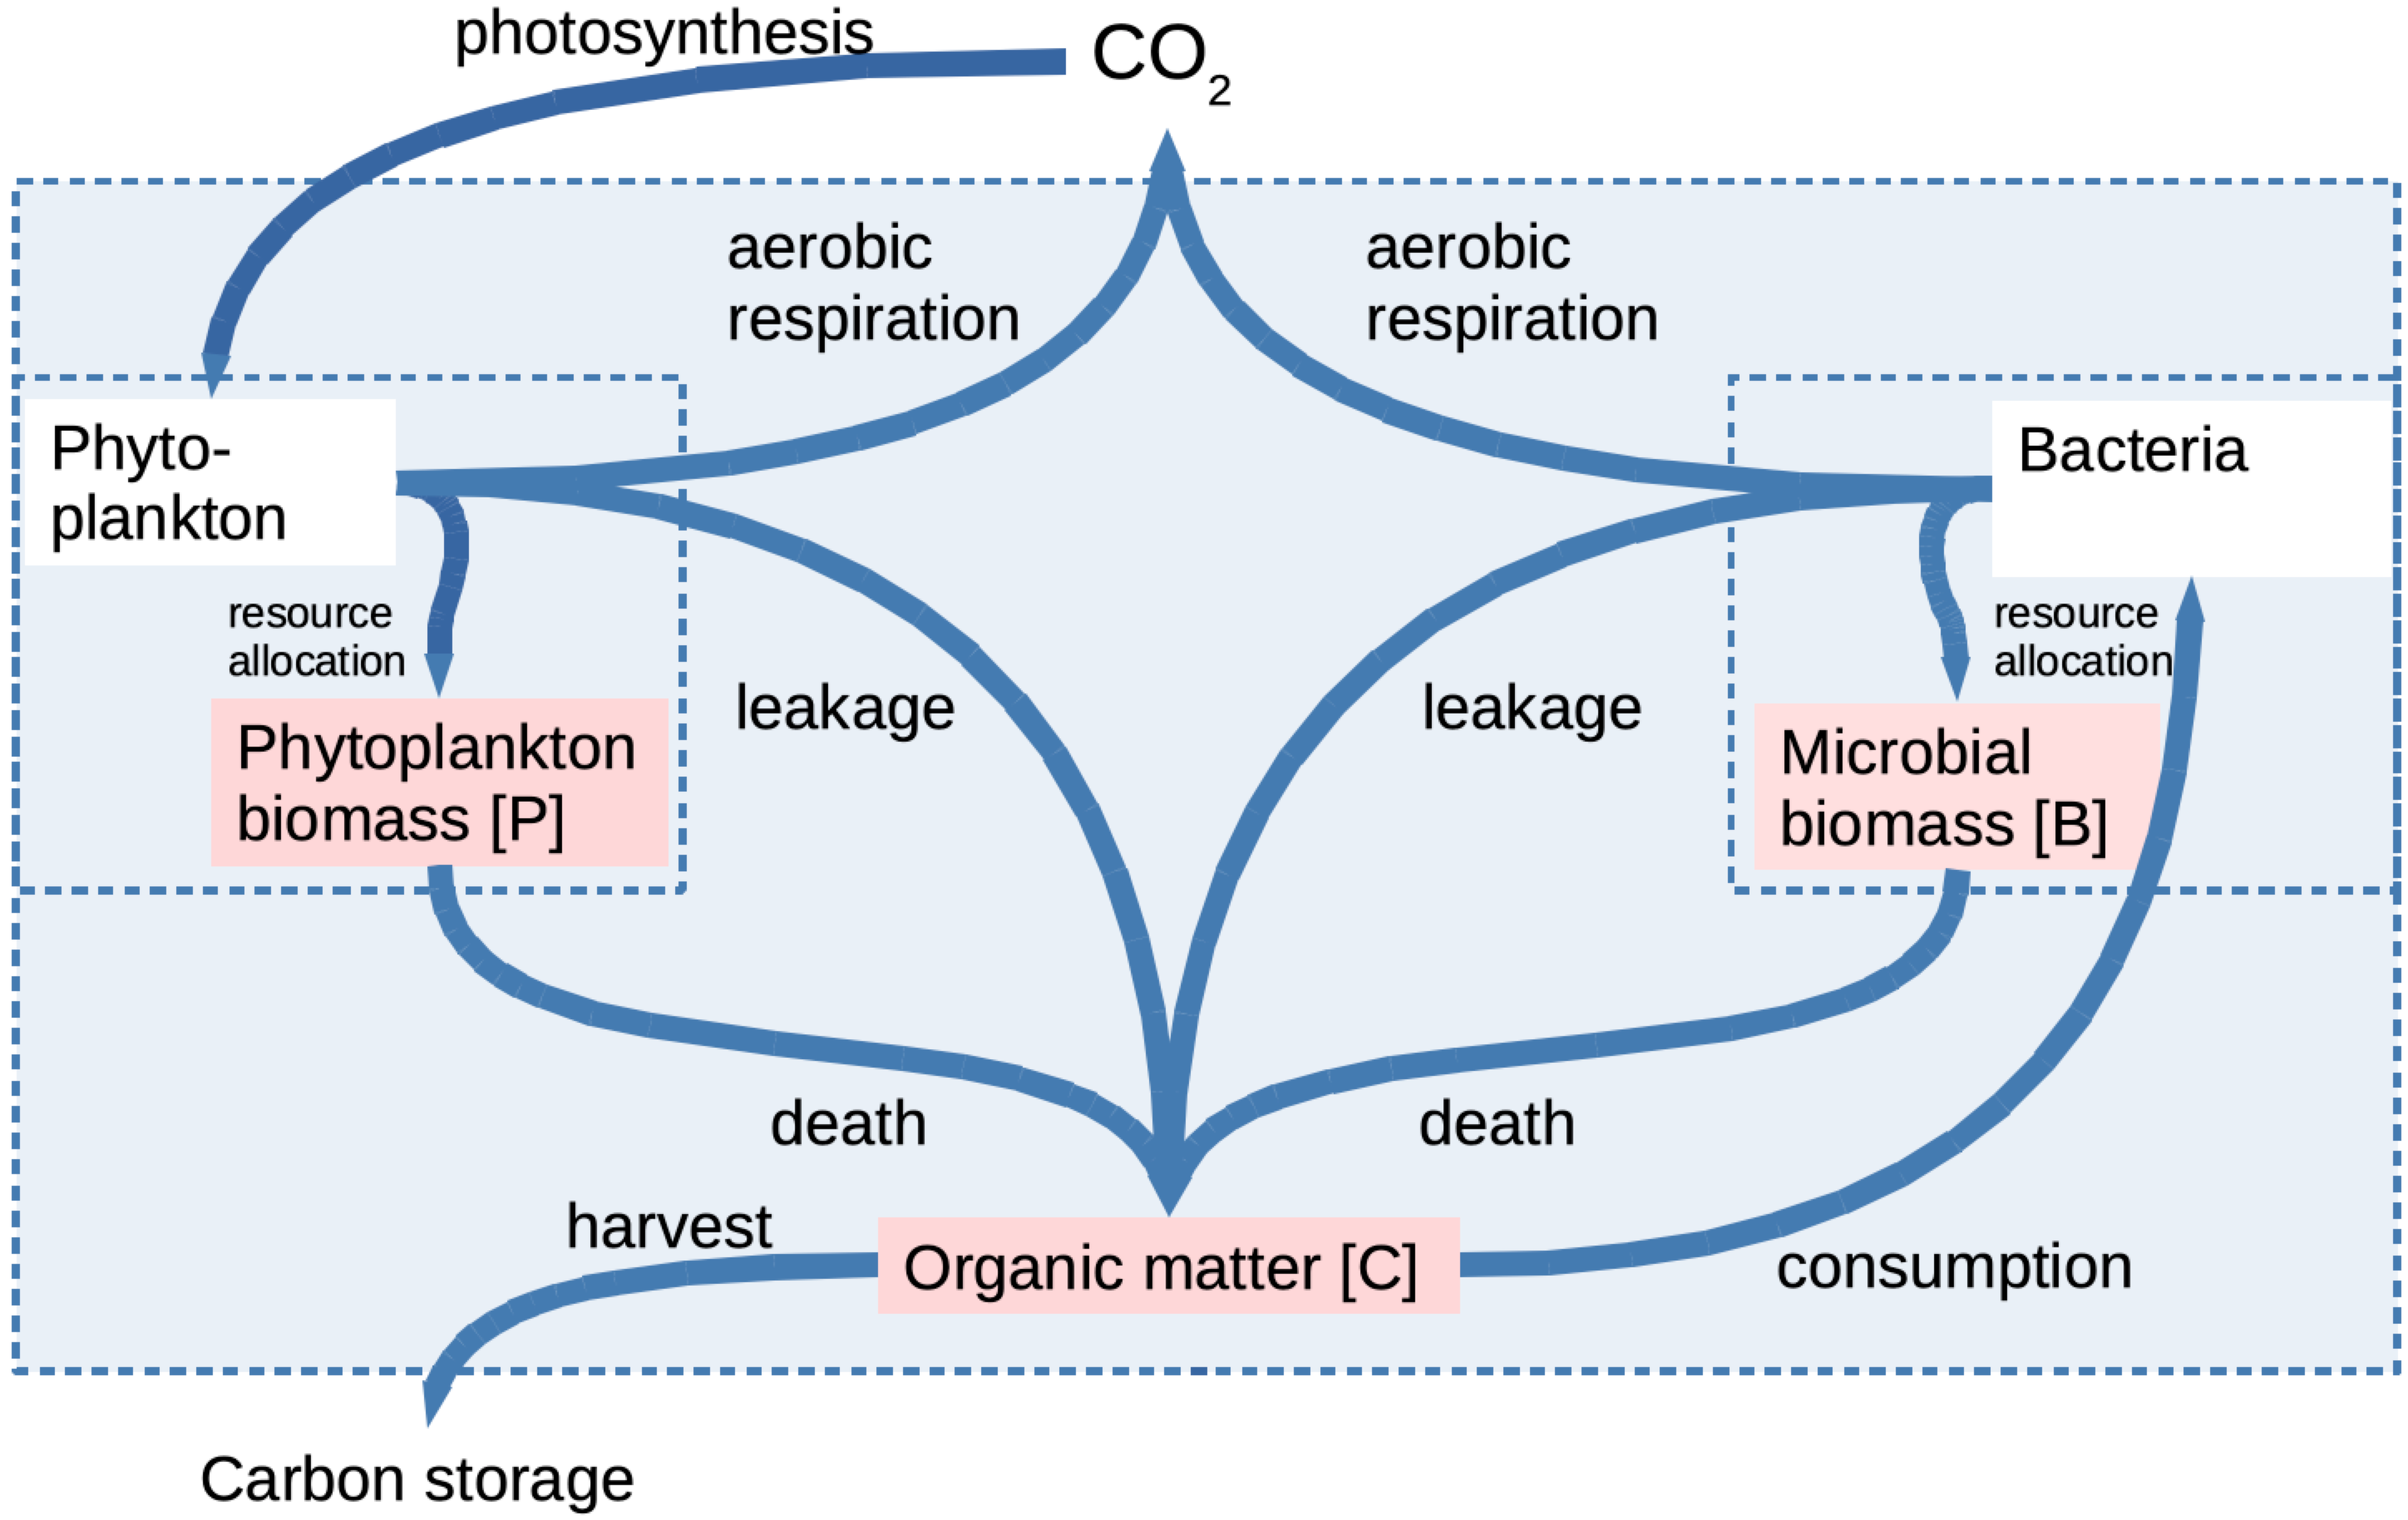
\includegraphics[width=.8\linewidth]{thesisSec/model.png}
    \caption[Model visualization]{Classification of dominant interactions in this project.  The two players shared all interactions with respective carbon pools but one, which was the energy acquiring method.}
    \label{modelInWord}
\end{figure}

\begin{table}[H]
    \centering
    \caption[Algebra variables definitions]{Table showing definition of variables used in the ODE system}
    \csvautotabular[]{thesisSec/varTab.csv}
    \label{varInTab}
\end{table}

\begin{table}[H]
    \centering
    \caption[Processes in algebra terms]{Table showing processes in Fig.\ref{modelInWord} direct translation into mathematical terms}
    \csvautotabular[]{thesisSec/termTab.csv}
    \label{termInTab}
\end{table}

\begin{equation*}\left\{\begin{array}{rl}
    C'(t) &= \ePR(1-\eP)\cdot\gP\cdot P +\aP\cdot P^2 +(\eBR(1-\eB)-1)\cdot\gB\cdot C\cdot B +\mB\cdot B -xC\\
    P'(t) &= \ePR\cdot\eP\cdot\gP\cdot P -\aP\cdot P^2\\
    B'(t) &= \eBR\cdot\eB\cdot\gB\cdot C\cdot B -\mB\cdot B
\end{array}\right.\end{equation*}

\end{document}